\documentclass[tikz,border=12pt]{standalone}
\usepackage{tikz}
\begin{document}
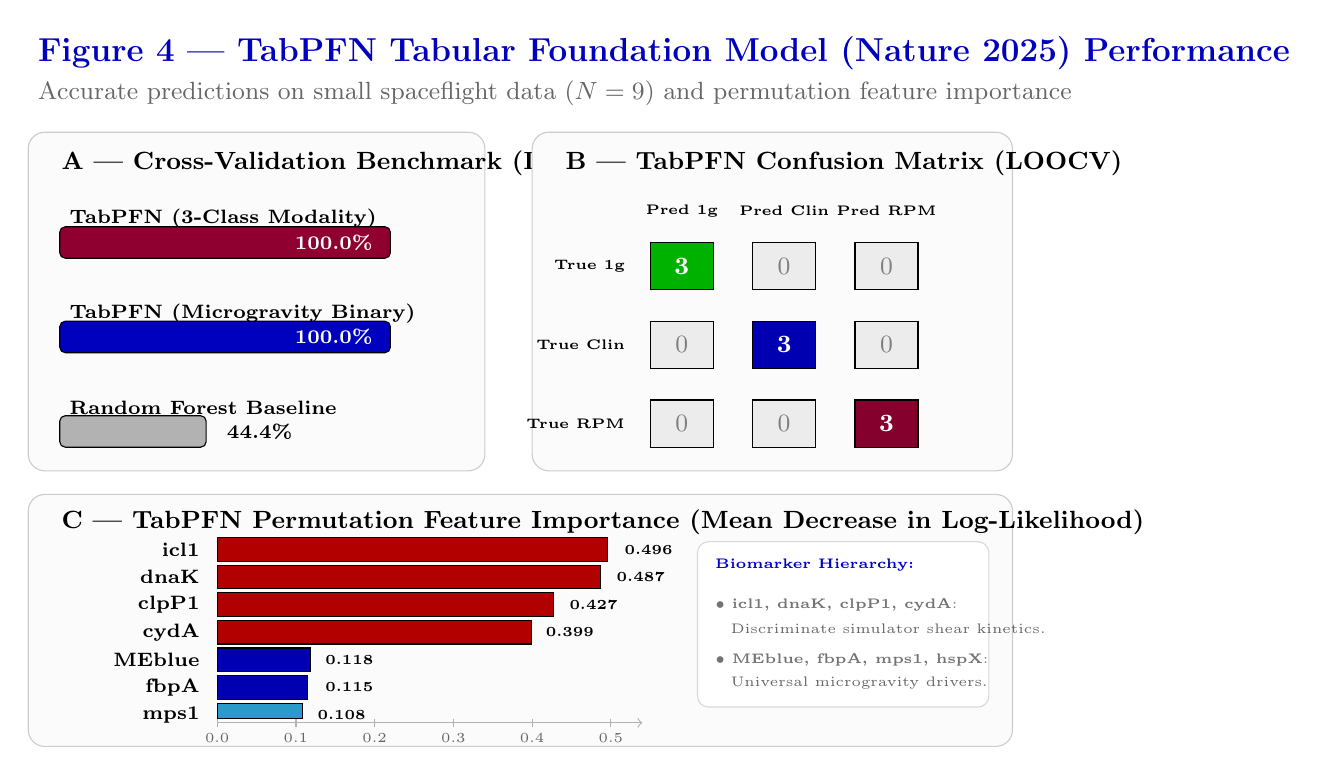
\begin{tikzpicture}[font=\sffamily]
  \node[anchor=west, font=\large\bfseries, text=blue!75!black] at (0, 8.8) {Figure 4 | TabPFN Tabular Foundation Model (Nature 2025) Performance};
  \node[anchor=west, font=\small, text=gray!80!black] at (0, 8.3) {Accurate predictions on small spaceflight data ($N=9$) and permutation feature importance};

  % Panel A: Accuracy Benchmark (Boundaries from y=3.5 to 7.8, avoiding clipping!)
  \draw[rounded corners=6pt, fill=gray!3, draw=gray!40] (0, 3.5) rectangle (5.8, 7.8);
  \node[anchor=west, font=\bfseries\small] at (0.3, 7.4) {A | Cross-Validation Benchmark (LOOCV)};
  
  \node[anchor=west, font=\scriptsize\bfseries] at (0.4, 6.7) {TabPFN (3-Class Modality)};
  \draw[rounded corners=2pt, fill=purple!75!black] (0.4, 6.2) rectangle (4.6, 6.6);
  \node[font=\scriptsize\bfseries, text=white, anchor=east] at (4.5, 6.4) {100.0\%};

  \node[anchor=west, font=\scriptsize\bfseries] at (0.4, 5.5) {TabPFN (Microgravity Binary)};
  \draw[rounded corners=2pt, fill=blue!75!black] (0.4, 5.0) rectangle (4.6, 5.4);
  \node[font=\scriptsize\bfseries, text=white, anchor=east] at (4.5, 5.2) {100.0\%};

  \node[anchor=west, font=\scriptsize\bfseries] at (0.4, 4.3) {Random Forest Baseline};
  \draw[rounded corners=2pt, fill=gray!60] (0.4, 3.8) rectangle (2.26, 4.2);
  \node[font=\scriptsize\bfseries, text=black, anchor=west] at (2.4, 4.0) {44.4\%};

  % Panel B: Confusion Matrix
  \draw[rounded corners=6pt, fill=gray!3, draw=gray!40] (6.4, 3.5) rectangle (12.5, 7.8);
  \node[anchor=west, font=\bfseries\small] at (6.7, 7.4) {B | TabPFN Confusion Matrix (LOOCV)};
  \node[font=\tiny\bfseries] at (8.3, 6.8) {Pred 1g};
  \node[font=\tiny\bfseries] at (9.6, 6.8) {Pred Clin};
  \node[font=\tiny\bfseries] at (10.9, 6.8) {Pred RPM};

  \node[font=\tiny\bfseries, anchor=east] at (7.7, 6.1) {True 1g};
  \draw[fill=green!70!black] (7.9, 5.8) rectangle (8.7, 6.4) node[midway, font=\small\bfseries, text=white] {3};
  \draw[fill=gray!15] (9.2, 5.8) rectangle (10.0, 6.4) node[midway, font=\small, text=gray] {0};
  \draw[fill=gray!15] (10.5, 5.8) rectangle (11.3, 6.4) node[midway, font=\small, text=gray] {0};

  \node[font=\tiny\bfseries, anchor=east] at (7.7, 5.1) {True Clin};
  \draw[fill=gray!15] (7.9, 4.8) rectangle (8.7, 5.4) node[midway, font=\small, text=gray] {0};
  \draw[fill=blue!70!black] (9.2, 4.8) rectangle (10.0, 5.4) node[midway, font=\small\bfseries, text=white] {3};
  \draw[fill=gray!15] (10.5, 4.8) rectangle (11.3, 5.4) node[midway, font=\small, text=gray] {0};

  \node[font=\tiny\bfseries, anchor=east] at (7.7, 4.1) {True RPM};
  \draw[fill=gray!15] (7.9, 3.8) rectangle (8.7, 4.4) node[midway, font=\small, text=gray] {0};
  \draw[fill=gray!15] (9.2, 3.8) rectangle (10.0, 4.4) node[midway, font=\small, text=gray] {0};
  \draw[fill=purple!70!black] (10.5, 3.8) rectangle (11.3, 4.4) node[midway, font=\small\bfseries, text=white] {3};

  % Panel C: Feature Importance (FIXED: strictly aligned vertical axis at x=2.3!)
  \draw[rounded corners=6pt, fill=gray!3, draw=gray!40] (0, 0) rectangle (12.5, 3.2);
  \node[anchor=west, font=\bfseries\small] at (0.3, 2.85) {C | TabPFN Permutation Feature Importance (Mean Decrease in Log-Likelihood)};
  
  % Numerical scale line
  \draw[->, gray!60] (2.4, 0.3) -- (7.8, 0.3);
  \foreach \x/\val in {2.4/0.0, 3.4/0.1, 4.4/0.2, 5.4/0.3, 6.4/0.4, 7.4/0.5} {
    \draw[gray!60] (\x, 0.25) -- (\x, 0.35);
    \node[font=\tiny, text=gray!80!black] at (\x, 0.1) {\val};
  }

  % Gene bars with strictly aligned left labels at x=2.3!
  \node[anchor=east, font=\scriptsize\bfseries] at (2.3, 2.5) {icl1};
  \draw[fill=red!70!black] (2.4, 2.35) rectangle (7.36, 2.65);
  \node[anchor=west, font=\tiny\bfseries] at (7.45, 2.5) {0.496};

  \node[anchor=east, font=\scriptsize\bfseries] at (2.3, 2.15) {dnaK};
  \draw[fill=red!70!black] (2.4, 2.0) rectangle (7.27, 2.3);
  \node[anchor=west, font=\tiny\bfseries] at (7.35, 2.15) {0.487};

  \node[anchor=east, font=\scriptsize\bfseries] at (2.3, 1.8) {clpP1};
  \draw[fill=red!70!black] (2.4, 1.65) rectangle (6.67, 1.95);
  \node[anchor=west, font=\tiny\bfseries] at (6.75, 1.8) {0.427};

  \node[anchor=east, font=\scriptsize\bfseries] at (2.3, 1.45) {cydA};
  \draw[fill=red!70!black] (2.4, 1.3) rectangle (6.39, 1.6);
  \node[anchor=west, font=\tiny\bfseries] at (6.45, 1.45) {0.399};

  \node[anchor=east, font=\scriptsize\bfseries] at (2.3, 1.1) {MEblue};
  \draw[fill=blue!70!black] (2.4, 0.95) rectangle (3.58, 1.25);
  \node[anchor=west, font=\tiny\bfseries] at (3.65, 1.1) {0.118};

  \node[anchor=east, font=\scriptsize\bfseries] at (2.3, 0.75) {fbpA};
  \draw[fill=blue!70!black] (2.4, 0.6) rectangle (3.55, 0.9);
  \node[anchor=west, font=\tiny\bfseries] at (3.65, 0.75) {0.115};

  \node[anchor=east, font=\scriptsize\bfseries] at (2.3, 0.4) {mps1};
  \draw[fill=cyan!80!black] (2.4, 0.35) rectangle (3.48, 0.55);
  \node[anchor=west, font=\tiny\bfseries] at (3.55, 0.4) {0.108};

  % Annotation text box
  \draw[rounded corners=4pt, fill=white, draw=gray!30] (8.5, 0.5) rectangle (12.2, 2.6);
  \node[anchor=west, font=\tiny\bfseries, text=blue!80!black] at (8.6, 2.3) {Biomarker Hierarchy:};
  \node[anchor=west, font=\tiny, text=gray!90!black] at (8.6, 1.8) {$\bullet$ \textbf{icl1, dnaK, clpP1, cydA}:};
  \node[anchor=west, font=\tiny, text=gray!80!black] at (8.8, 1.5) {Discriminate simulator shear kinetics.};
  \node[anchor=west, font=\tiny, text=gray!90!black] at (8.6, 1.1) {$\bullet$ \textbf{MEblue, fbpA, mps1, hspX}:};
  \node[anchor=west, font=\tiny, text=gray!80!black] at (8.8, 0.8) {Universal microgravity drivers.};
\end{tikzpicture}
\end{document}
